%"###############################################
%
% IPSS
%
%###############################################

Dans l’analyse suivante nous souhaitons observer la distribution des variables IPSS QoL et Qmax sur les différentes itérations temporelles fournies. L’objectif est de voir (pour l’ensemble des patients utilisant l’une des trois techniques) comment cette distribution évolue. 

\subsubsection{IPSS sur 18 mois }

RTUPB est une table composée de 36 patients. 
	
\begin{figure}[H]
\centering
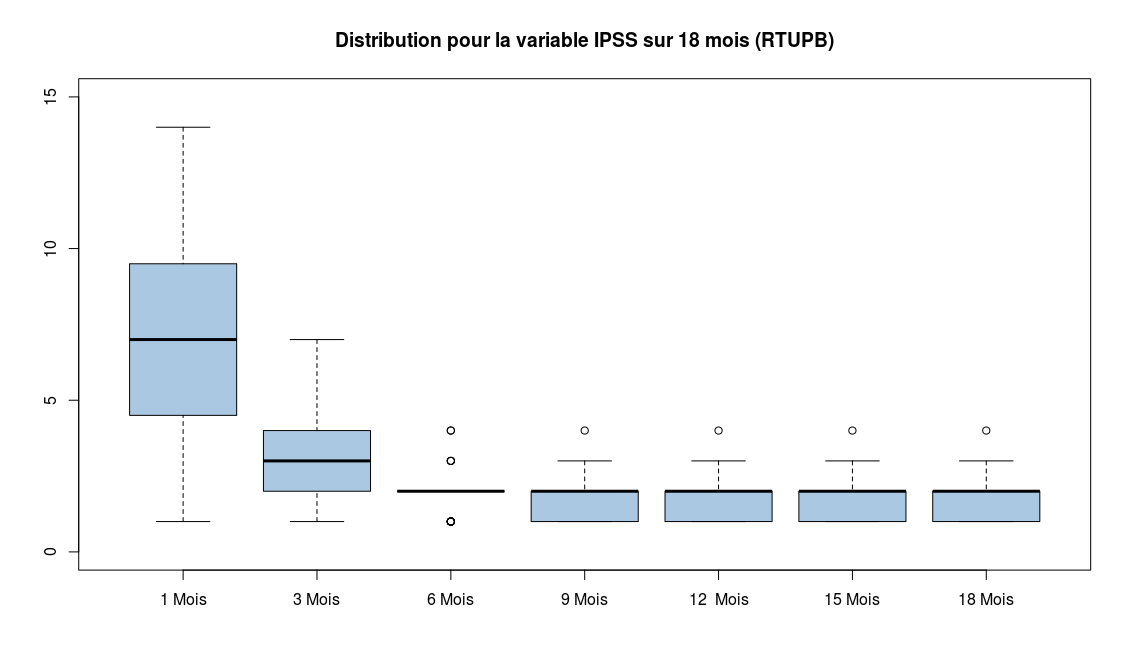
\includegraphics[width=0.75\textwidth]{../Fig/RTUPB/rtupb-boxplot-post-ipss}
\caption{RTUPB / IPSS sur 18 mois}
\end{figure}	
	
\begin{figure}[H]
\centering
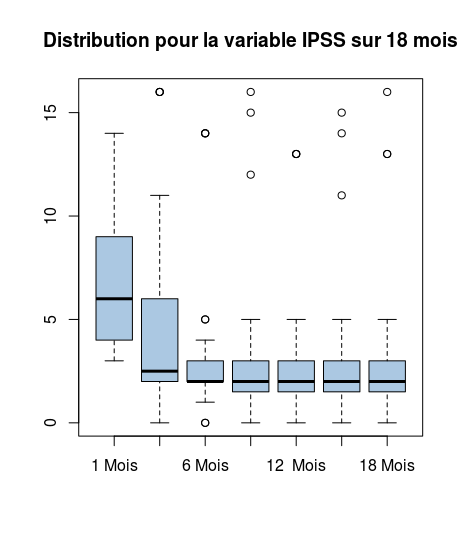
\includegraphics[width=0.75\textwidth]{../Fig/VPPBS/vppbs-boxplot-post-ipss}
\caption{VPPBS/IPSS sur 18 mois}
\end{figure}


\begin{figure}[H]
\centering
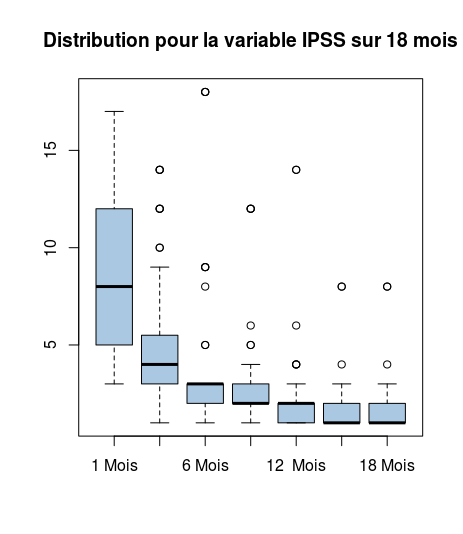
\includegraphics[width=0.75\textwidth]{../Fig/VAPOR/vapor-boxplot-post-ipss}
\caption{VAPOR/IPSS}
\end{figure}

%
%##########################
%# CONCLUSION
%##########################

Pour IPSS, l’on observe pour les trois techniques une décroissance de la valeur médiane dès le troisième mois. Dans le cadre de VAPOR et VPPBS, certains « outliers » sont présents (et ce sur l’ensemble des itérations dans le cadre de VPPBS ces « outliers » ont encore des valeurs très fortes même à partir du 18\up{ième} mois.  RTUPB  semble avoir une variance homogène à partir du 9\up{ième} mois. Si VAPOR laisse apparaître des « ouliers », la valeur médiane termine plus bas que les deux autres techniques. 
